\documentclass[a4paper,12pt]{paper}

\usepackage{mycommands}


\begin{document}

\title{Lecture 12: Finite Elasticity}
\author{David Al-Attar \\ Michaelmas Term, \the\year}



\maketitle


\section*{Outline and motivation}
In this lecture, we derive the equations of motion for an elastic body. These equations provide a good though not
complete model for understanding seismic wave propagation and other related topics in geophysics. Most of you will
have encountered elasticity within earlier courses, but here we will go back to first principles. In particular, we
discuss \textbf{finite elasticity}, by which we mean that there is no assumption that the deformation remains small.
Within later applications it will actually be sufficient to consider linearised motions about an equilibrium state, but
by starting with the exact theory it is easier to appreciate the underlying physics.

\section*{Basic definitions}
We start by considering the kinematics of a solid body. At an instant in time, $t$, the body occupies a subset $M_{t}$ 
of physical space, $\mathbb{R}^{3}$. A useful way to describe the motion is through the introduction of a \textbf{reference body}, 
$M$. Each point $\mathbf{x}$ in the reference body corresponds to a unique particle. At time $t$, the particle $\mathbf{x}$ 
sits at a point in physical space that we denote by $\bphi(\mathbf{x},t)$. In this manner we see that the evolution of the 
body is completely described by this time-dependent mapping, $\bphi(\cdot,t)$, from the reference body into physical space.
We will call $\bphi$ the \textbf{motion} of the body, this being the ``field'' within this classical field theory. We will not
consider motions for which the body is torn or fractured. As a result, we suppose that $\bphi$ is continuously differentiable,
and that at each fixed time, $t$, it establishes a one-to-one correspondence between $M$ and $M_{t}$. These ideas are summarised 
graphically in Fig.~\ref{fig:1}.


\begin{figure}[ht]
     \centering
     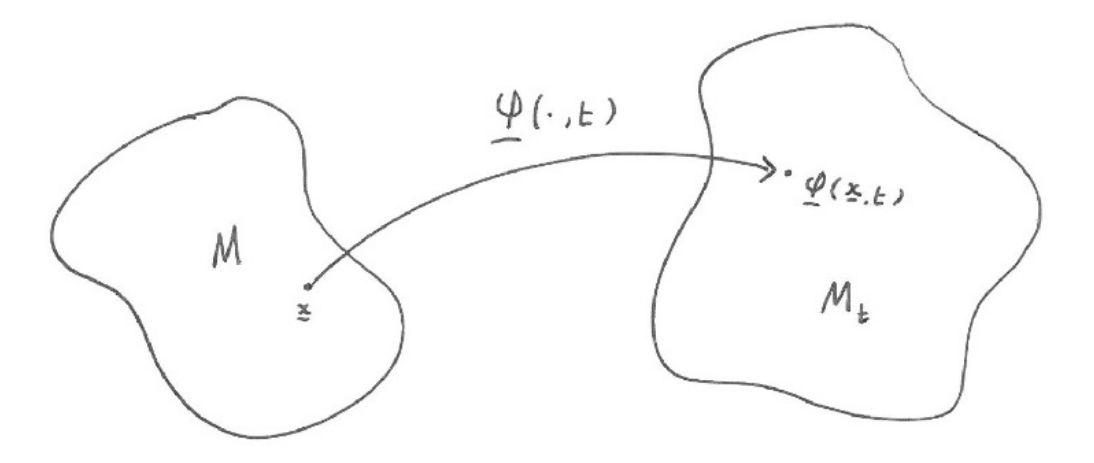
\includegraphics[width=0.7\textwidth]{figures/L1F1.png} 
     \caption{A schematic illustration of the mapping from the reference body $M$ into the body's instantaneous position in physical space.}
     \label{fig:1}
 \end{figure}

In making these definitions we have not specified how the reference body is chosen. Indeed, it turns out that there
are infinitely many ways of doing this. Nevertheless, a common approach is to 
let points in the reference body correspond to the position of the particles at some reference time, $t_{0}$. 
Having done this, we then have
\begin{equation}
\bphi(\mathbf{x},t_{0})=\mathbf{x},
\label{eq:1}
\end{equation}
for all $\mathbf{x}$. There are circumstances in which it is useful to select a different reference body, but 
we will not worry about that within this course. 

\section*{Velocity, deformation gradient, and Jacobian}
If we fix attention on a particle $\mathbf{x}$, then the function $t\mapsto\bphi(\mathbf{x},t)$ describes its 
trajectory through space. Differentiating with respect to time, we obtain the \textbf{referential velocity}
\begin{equation}
v_{i}(\mathbf{x},t)=\frac{\partial\varphi_{i}}{\partial t}(\mathbf{x},t).
\label{eq:2}
\end{equation}
Note that this is the velocity of a fixed particle, and not that at a fixed spatial point. This differs from what is commonly 
done in fluid mechanics. In what follows, we will generally drop the term ``referential'' and just say ``velocity'' for this 
vector field\footnote{I prefer the descriptive terms ``referential'' and ``spatial'' to describe the two means by which quantities can be 
described within a continuum. Some authors instead use ``Lagrangian'' and ``Eulerian'' for these concepts, though
 both perspectives were introduced by Euler. }. 

A second quantity that will be important is the \textbf{deformation gradient}, $\mathbf{F}$, which is defined by
\begin{equation}
F_{ij}=\frac{\partial\varphi_{i}}{\partial x_{j}}.
\label{eq:3}
\end{equation}
Physically, the deformation gradient quantifies how the motion differs between nearby points in the reference body. For 
example, if we consider particles $\mathbf{x}$ and $\mathbf{x}+\delta\mathbf{x}$ with $\delta\mathbf{x}$ small, then we can 
use a Taylor expansion to obtain
\begin{equation}
\varphi_{i}(\mathbf{x}+\delta\mathbf{x},t)=\varphi_{i}(\mathbf{x},t)+F_{ij}(\mathbf{x},t)\delta x_{j}+\cdots,
\label{eq:4}
\end{equation}
which is accurate to first-order in $\delta\mathbf{x}$. The deformation gradient is related to, but not identical with,
the concept of \textbf{strain}, with this correspondence discussed further in the next lecture.

Because we have assumed that the motion establishes a one-to-one correspondence between $M$ and $M_{t}$ at each time, it can 
be shown that $\mathbf{F}(\mathbf{x},t)$ is an invertible matrix at each point.\footnote{This follows from a result known as 
the \textbf{inverse function theorem}.} The determinant of the deformation gradient is known as the \textbf{Jacobian} of the
motion, and is written
\begin{equation}
J(\mathbf{x},t)=\det\mathbf{F}(\mathbf{x},t).
\label{eq:5}
\end{equation}
Invertibility of the deformation gradient implies that $J$ is never equal to zero, while continuity of $J$, which follows 
from the continuous differentiability of $\bphi$, implies that it is of one sign throughout the body. We will assume that $J$ is always positive. This implies in particular that a right-handed set of 
basis vectors in $M$ is mapped to a right-handed set of basis vectors in $M_{t}$.

Consider a function $f$ defined in the instantaneous body $M_{t}$, and its integral
\begin{equation}
I=\int_{M_{t}}f(\mathbf{y})\dd^{3}\mathbf{y}.
\label{eq:6}
\end{equation}
Using the motion at this instant in time, we can change variables to write the integral as one over the reference body
\begin{equation}
I=\int_{M}f[\bphi(\mathbf{x},t)]J(\mathbf{x},t)\dd^{3}\mathbf{x}.
\label{eq:7}
\end{equation}
This ability to easily transform integrals between the instantaneous and reference bodies will be very useful in what follows.


\section*{Conservation of mass}
Let $U$ be a subset of the reference body and $U_{t}$ the region of physical space it occupies at time $t$. The mass of this 
sub-body can be written
\begin{equation}
\int_{U_{t}}\varrho(\mathbf{y},t)\dd^{3}\mathbf{y},
\label{eq:8}
\end{equation}
where $\varrho(\mathbf{y},t)$ is the \textbf{spatial density} at the point $\mathbf{y}$ in $M_{t}$ at time $t$. During the deformation matter is 
neither created nor destroyed. This means that the mass of this arbitrary sub-body is constant, and hence 
\begin{equation}
\frac{\ddns}{\ddns t}\int_{U_{t}}\varrho(\mathbf{y},t)\dd^{3}\mathbf{y}=0.
\label{eq:9}
\end{equation}
To simplify this expression we use the motion to transform the integration in eq.(\ref{eq:9}) to the reference body
\begin{equation}
\frac{\ddns}{\ddns t}\int_{U}J(\mathbf{x},t)\varrho[\bphi(\mathbf{x},t),t]\dd^{3}\mathbf{x}=0.
\label{eq:10}
\end{equation}
This integral is over a fixed domain, and so we can interchange the order of differentiation and integration. Furthermore, as 
$U$ is an arbitrary subset of $M$, the resulting equality can hold for every such $U$ if and only if
\begin{equation}
\frac{\partial}{\partial t}\{J(\mathbf{x},t)\varrho[\bphi(\mathbf{x},t),t]\}=0.
\label{eq:11}
\end{equation}
It follows that we can introduce a time-independent \textbf{referential density} $\rho$ such that
\begin{equation}
\rho(\mathbf{x})=J(\mathbf{x},t)\varrho[\bphi(\mathbf{x},t),t].
\label{eq:12}
\end{equation}
This is a statement of mass conservation expressed within the reference body. Note that if the reference body is chosen such 
that eq.(\ref{eq:1}) holds at some time $t=t_{0}$ then at this time eq.(\ref{eq:12}) simplifies to
\begin{equation}
\rho(\mathbf{x})=\varrho(\mathbf{x},t_{0}).
\label{eq:13}
\end{equation}
Thus, when using this common choice of reference body, the referential density is precisely the density at the reference time.

\section*{Kinetic energy}
By analogy with particle mechanics, the \textbf{kinetic energy density} of the body, measured per unit volume within the reference body $M$, is defined as
\begin{equation}
\frac{1}{2}\rho(\mathbf{x})\|\mathbf{v}(\mathbf{x},t)\|^{2},
\label{eq:14}
\end{equation}
and summing up such contributions, we see that the total kinetic energy can be written
\begin{equation}
\mathcal{T}(t)=\frac{1}{2}\int_{M}\rho(\mathbf{x})\|\mathbf{v}(\mathbf{x},t)\|^{2}\dd^{3}\mathbf{x}.
\label{eq:15}
\end{equation}


\section*{Potential energy}
What should the potential energy of an elastic body look like? The basic idea is that the body has a preferred shape and/or volume, 
and that energy is required to deform the body away from this equilibrium state. As a starting point we assume that the 
potential energy can be expressed in the form
\begin{equation}
\mathcal{V}(t)=\int_{M}W[\mathbf{x},t,\bphi(\mathbf{x},t),\mathbf{F}(\mathbf{x},t)]\dd^{3}\mathbf{x},
\label{eq:16}
\end{equation}
where $W$ is a \textbf{potential energy density} measured per unit volume within the reference body. This is not the most general form 
that the potential energy could take, but defines what is known as a \textbf{simple hyperelastic body}. That a body is 
\textbf{hyperelastic} means that it has a well-defined potential energy. A consequence of this assumption -- that you will establish 
in the first problem set -- is that energy is conserved during the deformation of the body, and hence within this theory
we are discounting dissipative processes\footnote{The situation is analogous to particle mechanics restricted to the case of 
conservative forces, i.e., those forces that are derived from a potential energy.}.
Energy dissipation is relevant to seismology, but it 
is a relatively minor effect that we will neglect in this course. The term \textbf{simple} in the above context means that the 
potential energy density at a point, $\mathbf{x}$, depends only on the motion and the deformation gradient at the same point. 
By contrast, we might have allowed the potential energy density to depend on higher-order spatial derivatives of the motion, 
or on the motion in some non-local manner. But there seems to be no need for such generalisations for geophysical 
applications. 


\subsection*{Simplifying the potential energy using symmetries}
Having accepted the form of the potential energy in eq.(\ref{eq:16}), we are now in a position to obtain the equations of 
motion using Hamilton's principle. Before doing this, the form of the potential energy density can 
be simplified by imposing certain physical constraints:

\begin{enumerate}
    \item[(i)] \textbf{Time-translation invariance.} Consider a motion $\bphi(\mathbf{x},t)$ and its time-translation 
    $\bphi^{\prime}(\mathbf{x},t)=\bphi(\mathbf{x},t-\tau)$ for some $\tau$. The second motion takes 
    exactly the same form but is just shifted in time, and hence it is natural to require that their respective 
    potential energies satisfy
    \begin{equation}
    \mathcal{V}^{\prime}(t)=\mathcal{V}(t-\tau).
    \label{eq:17}
    \end{equation}
    This condition is automatically met if the potential energy density has no explicit dependence on time, and hence we simplify its form to
    \begin{equation}
    \mathcal{V}(t)=\int_{M}W[\mathbf{x},\bphi(\mathbf{x},t),\mathbf{F}(\mathbf{x},t)]\dd^{3}\mathbf{x}.
    \label{eq:18}
    \end{equation}
    The necessity of this condition can also be established.

    \item[(ii)] \textbf{Invariance under rigid body motions.} As stated above, an elastic body has a preferred shape and/or volume, 
    and the potential energy is associated with deformations of the body away from this. Motions that do not alter its shape nor 
    volume should not, therefore, be associated with a change in potential energy. Within Euclidean space, motions that do 
    not change the relative lengths between points arise through a combination of rotations and translations. If $\bphi$ 
    is a motion of the body, we can define a second motion $\bphi^{\prime}$ by setting
    \begin{equation}
    \bphi^{\prime}(\mathbf{x},t)=\mathbf{a}(t)+\mathbf{Q}(t)\bphi(\mathbf{x},t),
    \label{eq:19}
    \end{equation}
    where $\mathbf{a}(t)$ is a time-dependent translation vector and $\mathbf{Q}(t)$ a time-dependent rotation matrix. Because these motions differ only by a superimposed rigid body motion, they 
    must be associated with the same potential energy. Noting that $\mathbf{F}^{\prime}(\mathbf{x},t)=\mathbf{Q}(t)\mathbf{F}(\mathbf{x},t)$, 
    it follows that this invariance condition will be met so long as the potential energy density satisfies
    \begin{equation}
    W[\mathbf{x},\bphi(\mathbf{x},t),\mathbf{F}(\mathbf{x},t)]=W[\mathbf{x},\mathbf{a}(t)
    +\mathbf{Q}(t)\bphi(\mathbf{x},t),\mathbf{Q}(t)\mathbf{F}(\mathbf{x},t)].
    \label{eq:20}
    \end{equation}
    Again, necessity of this condition can also be proven. Setting $\mathbf{Q}(t)=\mathbf{1}$, this identity reduces to
    \begin{equation}
    W[\mathbf{x},\bphi(\mathbf{x},t),\mathbf{F}(\mathbf{x},t)]=W[\mathbf{x},\mathbf{a}(t)+\bphi(\mathbf{x},t),\mathbf{F}(\mathbf{x},t)].
    \label{eq:21}
    \end{equation}
    For fixed $(\mathbf{x}, t)$, we can vary $\mathbf{a}(t)$ such that the second argument on the right hand side takes any possible value.
     It follows that the potential energy density must be independent of its second argument. Given this result, it is useful to again 
     re-define the potential energy density to depend only on $\mathbf{x}$ and $\mathbf{F}(\mathbf{x},t)$, and having done this 
     the condition in eq.(\ref{eq:20}) reduces to
    \begin{equation}
    W[\mathbf{x},\mathbf{F}(\mathbf{x},t)]=W[\mathbf{x},\mathbf{Q}(t)\mathbf{F}(\mathbf{x},t)],
    \label{eq:22}
    \end{equation}
    for all deformation gradients, and all rotation matrices $\mathbf{Q}(t)$. This condition limits the allowable form of the potential
    energy density, and we will explore its consequences further within the next lecture.
\end{enumerate}
In summary, we find that the potential energy takes the simpler form
\begin{equation}
\mathcal{V}(t)=\int_{M}W[\mathbf{x},\mathbf{F}(\mathbf{x},t)]\dd^{3}\mathbf{x},
\label{eq:23}
\end{equation}
where $W$ is subject to eq.(\ref{eq:22}). Within continuum mechanics this potential energy density is  called the 
\textbf{strain energy function}, and this is the term we shall use from now on. The invariance of the potential energy under (i) time-translation, 
and (ii) superimposed rigid body motions, goes under the collective name of the principle of \textbf{material frame indifference}. This 
idea was developed by Clifford Truesdell and Walter Noll during the 1950s and 1960s, and plays a central role within all branches of theoretical continuum 
mechanics. Here we have only formulated this principle for a simple hyperelastic body, but it can be generalised to other types 
of material, and to incorporate thermodynamics and electromagnetism.

\section*{Hamilton's principle}
A Lagrangian density for a hyperelastic body is defined in the usual manner\footnote{For those with less experience with variational principles, 
the necessary ideas are developed here from first principles. But please ask in a supervision, or otherwise, if you would 
like any additional help with this material.} as the difference between the kinetic and potential energy densities
\begin{equation}
\mathcal{L}(\mathbf{x},t,\bphi,\mathbf{v},\mathbf{F})=\frac{1}{2}\rho(\mathbf{x})\|\mathbf{v}\|^{2}-W(\mathbf{x},\mathbf{F}),
\label{eq:24}
\end{equation}
while the associated action is
\begin{equation}
\mathcal{S}(\bphi)=\int_{0}^{T}\int_{M}\mathcal{L}[\mathbf{x},t,\bphi(\mathbf{x},t),\mathbf{v}(\mathbf{x},t),\mathbf{F}(\mathbf{x},t)]\dd^{3}\mathbf{x}\dd t,
\label{eq:25}
\end{equation}
where $[0, T]$ is the time interval of interest, and it is understood that the referential velocity and deformation 
gradient on the right hand side are those associated with the given motion. Note that the Lagrangian density in eq.(\ref{eq:24}) 
shows no explicit dependence on either $t$ or $\bphi$, but we shall 
retain this more general expression in what follows. Hamilton's principle states that the true motion is a stationary point 
of the action with respect to all smooth variations $\delta\bphi$ which satisfy the fixed end-point condition
\begin{equation}
\delta\bphi(\mathbf{x},0)=\delta\bphi(\mathbf{x},T)=\mathbf{0}.
\label{eq:26}
\end{equation}
Mathematically, this means that we require the first variation of the action
\begin{equation}
\delta\mathcal{S}=\lim_{h\rightarrow0}\frac{1}{h}[\mathcal{S}(\bphi+h~\delta\bphi)-\mathcal{S}(\bphi)]
\label{eq:27}
\end{equation}
vanish for all smooth variations $\delta\bphi$ satisfying eq.(\ref{eq:26}). We readily find that this 
first variation can be written
\begin{equation}
\delta\mathcal{S}=\int_{0}^{T}\int_{M}\left\{\frac{\partial\mathcal{L}}{\partial\varphi_{i}}\delta\varphi_{i}+
\frac{\partial\mathcal{L}}{\partial v_{i}}\delta v_{i}+\frac{\partial\mathcal{L}}{\partial F_{ij}}\delta F_{ij}\right\}\dd^{3}\mathbf{x}\dd t,
\label{eq:28}
\end{equation}
where the variations in the referential velocity and deformation gradient are given by
\begin{align}
\delta v_{i}&=\frac{\partial\delta\varphi_{i}}{\partial t}, \label{eq:29a}\\
\delta F_{ij}&=\frac{\partial\delta\varphi_{i}}{\partial x_{j}}, \label{eq:29b}
\end{align}
and we have suppressed all arguments for clarity. From the following identities
\begin{align}
\frac{\partial\mathcal{L}}{\partial v_{i}}\delta v_{i}&=\frac{\partial}{\partial t}\left(\frac{\partial\mathcal{L}}{\partial v_{i}}\delta\varphi_{i}
\right)-\frac{\partial}{\partial t}\left(\frac{\partial\mathcal{L}}{\partial v_{i}}\right)\delta\varphi_{i}, \label{eq:30}\\
\frac{\partial\mathcal{L}}{\partial F_{ij}}\delta F_{ij}&=\frac{\partial}{\partial x_{j}}\left(\frac{\partial\mathcal{L}}
{\partial F_{ij}}\delta\varphi_{i}\right)-\frac{\partial}{\partial x_{j}}\left(\frac{\partial\mathcal{L}}{\partial F_{ij}}\right)\delta\varphi_{i}, \label{eq:31}
\end{align}
along with eq.(\ref{eq:26}) and the divergence theorem, we obtain
\begin{equation}
\delta\mathcal{S}=\int_{0}^{T}\int_{M}\left\{\frac{\partial\mathcal{L}}{\partial\varphi_{i}}-
\frac{\partial}{\partial t}\left(\frac{\partial\mathcal{L}}{\partial v_{i}}\right)-\frac{\partial}{\partial x_{j}}
\left(\frac{\partial\mathcal{L}}{\partial F_{ij}}\right)\right\}\delta\varphi_{i}\dd^{3}\mathbf{x}\dd t+
\int_{0}^{T}\int_{\partial M}\frac{\partial\mathcal{L}}{\partial F_{ij}}\hat{n}_{j}\delta\varphi_{i}\dd S\dd t,
\label{eq:32}
\end{equation}
where $\hat{\mathbf{n}}$ denotes the outward unit normal vector to $\partial M$, and $\dd S$ is the surface element. 
As $\delta\bphi$ is arbitrary, this first variation can vanish only if the volume and boundary terms are 
independently equal to zero\footnote{If this statement is not obvious, then you might wish to ask in a supervision. But for the 
purposes of this course it is sufficient to know how to apply this method.}. Hamilton's principle, therefore, implies that 
the \textbf{Euler-Lagrange equations}
\begin{equation}
\frac{\partial\mathcal{L}}{\partial\varphi_{i}}-\frac{\partial}{\partial t}\left(\frac{\partial\mathcal{L}}{\partial v_{i}}\right)-\frac{\partial}{\partial x_{j}}\left(\frac{\partial\mathcal{L}}{\partial F_{ij}}\right)=0,
\label{eq:33}
\end{equation}
hold within the body, while we also have the \textbf{natural boundary conditions}
\begin{equation}
\frac{\partial\mathcal{L}}{\partial F_{ij}}\hat{n}_{j}=0,
\label{eq:34}
\end{equation}
on $\partial M$. Note that these boundary conditions are called ``natural'' because they have arisen directly from the 
variational principle, and not because of some prior restriction on the class of admissible motions.


For the Lagrangian density in eq.(\ref{eq:24}) we readily find that
\begin{align}
\frac{\partial\mathcal{L}}{\partial\varphi_{i}}&=0, \label{eq:35a}\\
\frac{\partial\mathcal{L}}{\partial v_{i}}&=\rho v_{i}, \label{eq:35b}\\
\frac{\partial\mathcal{L}}{\partial F_{ij}}&=-\frac{\partial W}{\partial F_{ij}}. \label{eq:35c}
\end{align}
The \textbf{first Piola-Kirchhoff stress tensor} is defined by
\begin{equation}
T_{ij}(\mathbf{x},t)=\frac{\partial W}{\partial F_{ij}}[\mathbf{x},\mathbf{F}(\mathbf{x},t)],
\label{eq:36}
\end{equation}
so that the Euler-Lagrange equations can be written
\begin{equation}
\rho\frac{\partial v_{i}}{\partial t}-\frac{\partial T_{ij}}{\partial x_{j}}=0,
\label{eq:37}
\end{equation}
while the boundary condition becomes
\begin{equation}
T_{ij}\hat{n}_{j}=0.
\label{eq:38}
\end{equation}
The vector $\mathbf{t}=\mathbf{T}\hat{\mathbf{n}}$ occurring in the boundary conditions is known as the \textbf{traction}. Within the 
first problem set you will see that it represents a \emph{surface force measured per unit area} within the reference body. 
Indeed, what the first Piola-Kirchhoff stress does is relate the orientation of a surface within the reference body 
to the force acting on the instantaneous image of that surface within physical space, this force being measured 
per unit area within the reference body. 

There are other stress tensors that can be defined. For example, within spatial descriptions of continuum mechanics, 
there is the \textbf{Cauchy stress tensor} which relates the orientation of surfaces in the instantaneous body 
to the force per unit area acting on this instantaneous surface. The Cauchy stress tensor is the one that 
is most commonly used within fluid mechanics (including in the earlier parts of this course). In the next lecture, 
we will see that within linearised theories about a stress-free equilibrium state the first Piola-Kirchhoff
stress and the Cauchy stress are equal, with this result accounting for the fact that their distinction 
is not made or emphasised within elementary courses on continuum mechanics. 


As a final comment, 
the equations of motion  are defined on the \emph{fixed} reference body, and hence we need not worry about applying 
boundary conditions on a moving boundary as is sometimes required in fluid mechanics problems that use a spatial formulation 
of continuum mechanics. This fact considerably simplifies 
the solution of free-boundary problems in elasticity, and is one of the reasons for working with a referential description 
of the motion.

\section*{What you need to know and be able to do}
\begin{enumerate}
    \item[(i)] Understand the terminology needed to describe the kinematics of an elastic body.
    \item[(ii)] Use the conservation of mass to derive the relation between the spatial and referential densities.
    \item[(iii)] State expressions for the kinetic and potential energies of a simple hyperelastic body, and 
    explain the underlying physical ideas and assumptions.
    \item[(iv)] Give a statement of Hamilton's principle in the context of finite elasticity, and use it to derive 
    the equations of motion and associated boundary conditions.
\end{enumerate}

\end{document}
